\section{Results and Analysis}


% \begin{table*}[t]
%     \centering
%     \caption{Comparison of Depression Detection Models}
%     \scalebox{0.9}{
%     \begin{tabular}{|l|l|l|c|l|l|l|}
%     \hline
%     \textbf{Author} & \textbf{Dataset} & \textbf{Model} & \textbf{F1-score (\%)} & \makecell{\textbf{Speaker} \\ \textbf{Dependency}} & \textbf{Features} & \makecell{\textbf{Additional} \\ \textbf{Features}} \\
%     \hline
%     Gergo Gyori & DAIC & DT & 65 & Independent & MFCC & No \\
%     \hline
%     Gergo Gyori & EATD & DT & 68 & Independent & MFCC & No \\
%     \hline
%     Gergo Gyori & DAIC & TCC & 74 & Dependent & MFCC & No \\
%     \hline
%     Gergo Gyori & DAIC & TCC & 58 & Dependent & MFC & No \\
%     \hline
%     Gergo Gyori & DAIC & CNN & 50 & Independent & MFCC & No \\
%     \hline
%     Ishimaru et al. & DAIC & CNN & 96 & Dependent & MFCC & Yes \\
%     \hline
%     Ishimaru et al. & DAIC & CNN & 49 & Independent & MFCC & Yes \\
%     \hline
%     Yin et al. & DAIC & TCC & 93 & Dependent & MFCC & Yes \\
%     \hline
%     Homsiang et al. & DAIC & 1D CNN & 95 & Dependent & MFC & No \\
%     \hline
%     \label{tab:model-comparison}
%     \end{tabular}
%     }
% \end{table*}


\begin{table*}[t]
    \centering
    \caption{Comparison of Depression Detection Models}
    \scalebox{0.9}{
    \begin{tabular}{|l|l|l|c|l|l|l|}
    \hline
    \textbf{Author} & \textbf{Dataset} & \textbf{Model} & \textbf{F1-score (\%)} & \makecell{\textbf{Speaker} \\ \textbf{Dependency}} & \textbf{Features} & \makecell{\textbf{Additional} \\ \textbf{Features}} \\
    \hline
    Gyori & DAIC & DT & 65 & Independent & MFCC & No \\
    \hline
    Gyori & EATD & DT & 68 & Independent & MFCC & No \\
    \hline
    Gyori & DAIC & TCC & 74 & Dependent & MFCC & No \\
    \hline
    Gyori & DAIC & TCC & 58 & Dependent & MFC & No \\
    \hline
    Gyori & DAIC & CNN & 50 & Independent & MFCC & No \\
    \hline
    Ishimaru et al. & DAIC & CNN & 96 & Dependent & MFCC & Yes \\
    \hline
    Ishimaru et al. & DAIC & CNN & 49 & Independent & MFCC & Yes \\
    \hline
    Yin et al. & DAIC & TCC & 93 & Dependent & MFCC & Yes \\
    \hline
    Homsiang et al. & DAIC & 1D CNN & 95 & Dependent & MFC & No \\
    \hline
    \end{tabular}
    }
    \label{tab:model-comparison}
\end{table*}

\subsection{Analysis of Speaker Dependency}
A critical insight emerged during the analysis of different studies' performance metrics: the distinction between speaker dependent and independent approaches significantly impacts reported results. In \textit{speaker dependent} setups, different segments from the same participant's interview can appear in both training and test sets -- for example, various 30-second chunks from a single 5-minute interview might be distributed across both sets. While this ensures no exact duplicate segments exist between sets, the model can still learn speaker-specific characteristics.

In contrast, \textit{speaker independent} approaches maintain strict separation: all segments from a participant's interview are allocated either entirely to training or test sets. This previously unaddressed factor in my methodology explains the substantial performance differences observed in Table \ref{tab:model-comparison}, where speaker dependent approaches consistently show higher F1-scores compared to speaker independent setups. This finding highlights the importance of clearly specifying speaker dependency when reporting depression detection results.

\begin{figure}[H]
    \centering
    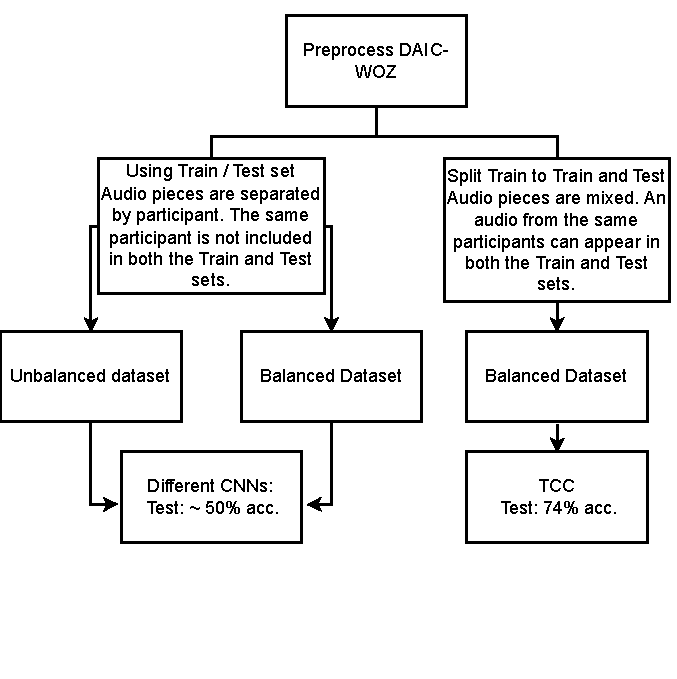
\includegraphics[width=0.45\textwidth]{vis_pdf/Train Test problem.drawio.pdf}
    \caption{Train/Test split strategies and their results (DAIC)}
    \label{fig:train_test_split_problems}
\end{figure}

This section presents the results of the experiments conducted in this study, organized into subsections focusing on specific aspects of the project. Initially, the performance of DT models is compared across the DAIC and EATD datasets. In the subsequent TCC section, only the DAIC dataset is used for evaluation. The different strategies are visualized on figure ~\ref{fig:train_test_split_problems}.




Table \ref{tab:model-comparison} provides a comparison of the models discussed in the literature, highlighting the differences in dataset, model, F1-score, split strategy, speaker dependency, features, and additional features. The models are evaluated based on their performance on the DAIC dataset, with the F1-score serving as the primary metric for comparison.



\subsection{Model Performance - DT}
While the models showcased performance on the DAIC dataset with an accuracy of 98.11\% on the training set (Tables \ref{table:classification_report_train_daic} and Figures \ref{fig:confusion_matrices_daic}, \ref{table:classification_report_dev_daic}), a significant drop in performance was observed on the development set.

Particularly, the development set for the DAIC dataset displayed only a 66\% accuracy (Table \ref{table:classification_report_dev_daic}), suggesting issues with the model's ability to generalize to new data. 

Similarly, for the EATD dataset, while the training results were promising with an accuracy of 87\% (Table \ref{table:classification_report_train_eatd}), the development set results were considerably lower, achieving only a 68\% accuracy (Table \ref{table:classification_report_dev_eatd}). This performance decrement underscores the necessity to consider alternative modeling strategies that might improve generalization across unseen datasets.


\begin{table}[H]
    \centering
    \caption{Classification Report on Training Set - DAIC}
    \scalebox{0.8}{% Scale the table to 50% of the original size
    \begin{tabular}{|c|c|c|c|c|}
    \hline
    \textbf{Class} & \textbf{Precision} & \textbf{Recall} & \textbf{F1-score} & \textbf{Support} \\ \hline
    0              & 0.97               & 1.00            & 0.99              & 76               \\ \hline
    1              & 1.00               & 0.93            & 0.97              & 30               \\ \hline
    \multicolumn{5}{|c|}{\textbf{Accuracy}: 0.98 \textbf{of} 106}                         \\ \hline
    \multicolumn{5}{|c|}{\textbf{Macro Avg}: Precision 0.99, Recall 0.97, F1-score 0.98} \\ \hline
    \multicolumn{5}{|c|}{\textbf{Weighted Avg}: Precision 0.98, Recall 0.98, F1-score 0.98} \\ \hline
    \end{tabular}}
    
    \label{table:classification_report_train_daic}
\end{table}


\begin{table}[H]
    \centering
    \caption{Classification Report on Development Set - DAIC}
    \scalebox{0.8}{% Scale the table to 50% of the original size
    \begin{tabular}{|c|c|c|c|c|}
    \hline
    \textbf{Class} & \textbf{Precision} & \textbf{Recall} & \textbf{F1-score} & \textbf{Support} \\ \hline
    0              & 0.76               & 0.65            & 0.70              & 20               \\ \hline
    1              & 0.53               & 0.67            & 0.59              & 12               \\ \hline
    \multicolumn{5}{|c|}{\textbf{Accuracy}: 0.66 \textbf{of} 32}                          \\ \hline
    \multicolumn{5}{|c|}{\textbf{Macro Avg}: Precision 0.65, Recall 0.66, F1-score 0.65} \\ \hline
    \multicolumn{5}{|c|}{\textbf{Weighted Avg}: Precision 0.68, Recall 0.66, F1-score 0.66} \\ \hline
    \end{tabular}}
    
    \label{table:classification_report_dev_daic}
\end{table}

\begin{figure}[H]
    \centering
    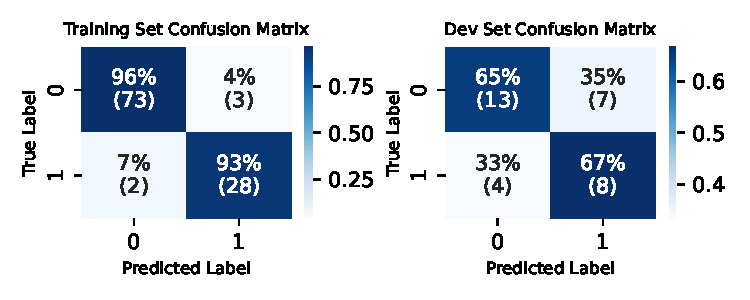
\includegraphics[width=0.45\textwidth]{vis_pdf/daic_all_confusion_matrices.pdf} % Adjust the scale to fit the page
    \caption{Confusion Matrices - DAIC}
    \label{fig:confusion_matrices_daic}
\end{figure}


%EATD

%TRAIN

\begin{table}[H]
    \centering
    \caption{Classification Report on Training Set - EATD}
    \scalebox{0.8}{% Scale the table to 80% of the original size
    \begin{tabular}{|c|c|c|c|c|}
    \hline
    \textbf{Class} & \textbf{Precision} & \textbf{Recall} & \textbf{F1-score} & \textbf{Support} \\ \hline
    0              & 0.96               & 0.84            & 0.90              & 56               \\ \hline
    1              & 0.74               & 0.93            & 0.82              & 27               \\ \hline
    \multicolumn{5}{|c|}{\textbf{Accuracy}: 0.87 \textbf{of} 83}                        \\ \hline
    \multicolumn{5}{|c|}{\textbf{Macro Avg}: Precision 0.85, Recall 0.88, F1-score 0.86} \\ \hline
    \multicolumn{5}{|c|}{\textbf{Weighted Avg}: Precision 0.89, Recall 0.87, F1-score 0.87} \\ \hline
    \end{tabular}}
    
    \label{table:classification_report_train_eatd}
\end{table}



\begin{table}[H]
    \centering
    \caption{Classification Report on Dev. Set- EATD}
    \scalebox{0.8}{% Scale the table to 80% of the original size
    \begin{tabular}{|c|c|c|c|c|}
    \hline
    \textbf{Class} & \textbf{Precision} & \textbf{Recall} & \textbf{F1-score} & \textbf{Support} \\ \hline
    0              & 0.71               & 0.88            & 0.79              & 52               \\ \hline
    1              & 0.54               & 0.27            & 0.36              & 26               \\ \hline
    \multicolumn{5}{|c|}{\textbf{Accuracy}: 0.68 \textbf{of} 78}                        \\ \hline
    \multicolumn{5}{|c|}{\textbf{Macro Avg}: Precision 0.62, Recall 0.58, F1-score 0.57} \\ \hline
    \multicolumn{5}{|c|}{\textbf{Weighted Avg}: Precision 0.65, Recall 0.68, F1-score 0.64} \\ \hline
    \end{tabular}}
    
    \label{table:classification_report_dev_eatd}
\end{table}


\begin{figure}[H]
\centering
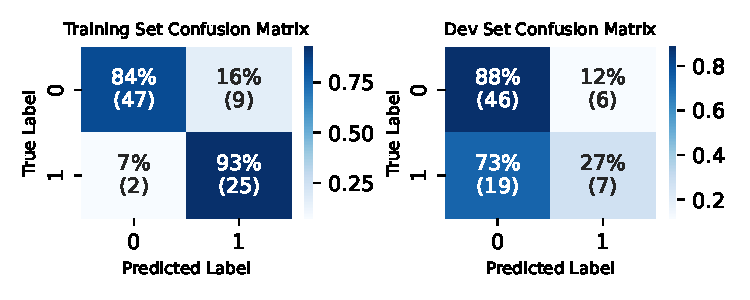
\includegraphics[width=0.45\textwidth]{vis_pdf/eatd_all_confusion_matrices.pdf} % Adjust the scale to fit the page
\caption{Confusion Matrices - EATD}
\label{fig:confusion_matrices_eatd}
\end{figure}

Training DT on both DAIC and EATD datasets revealed that ANOVA selected different top features for each dataset, indicating potential challenges in generalizing the model across different data conditions.

\subsection{Model Performance - CNN}

In my experiments with various CNN models described in the literature, the models consistently underperformed, achieving only 50\% accuracy on the development set (see Table \ref{tab:model-comparison}). A deeper investigation into the literature revealed a critical distinction: while speaker independent approaches (where participants' data is strictly separated between train and test sets) showed similar modest performance, models achieving high accuracy (>90\%) were predominantly using speaker dependent setups.

This performance gap is evident in Table \ref{tab:model-comparison}, where speaker dependent approaches by Ishimaru et al., Yin et al., and Homsiang et al. achieved F1-scores of 96\%, 93\%, and 95\% respectively, while speaker independent implementations, including our implementation, struggled to exceed 50\%. In speaker dependent setups, different segments from the same participant's interview were distributed between train and test sets, allowing models to learn individual speech characteristics rather than generalizable depression indicators.

The CNN models struggled to generalize when tasked with predicting new, unseen participants. The variance in accuracy across different CNN architectures is not discussed in this report. Instead, we focus on the results from the TCC model, detailed in Figure \ref{fig:confusion_matrices_TCC_daic}.
The training and validation accuracy and loss are depicted in Figure \ref{fig:training_TCC_daic}. The model underwent training for approximately 100 epochs, not to achieve the best possible accuracy but to demonstrate the model’s learning capability.
The model reached a 74\% accuracy on the development set, using a lightweight version of the architecture proposed by Yin et al \cite{yin2023depression}. The evaluation metrics presented are based on the model's performance at its peak accuracy.

\begin{figure}[H]
    \centering
    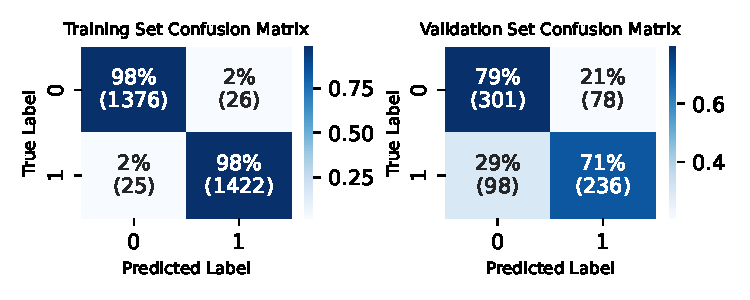
\includegraphics[width=0.45\textwidth]{vis_pdf/TCC_FINAL.pdf} % Adjust the scale to fit the page
    \caption{Confusion Matrices (Speaker Dependent - DAIC)}
    \label{fig:confusion_matrices_TCC_daic}
\end{figure}

\begin{figure}[H]
    \centering
    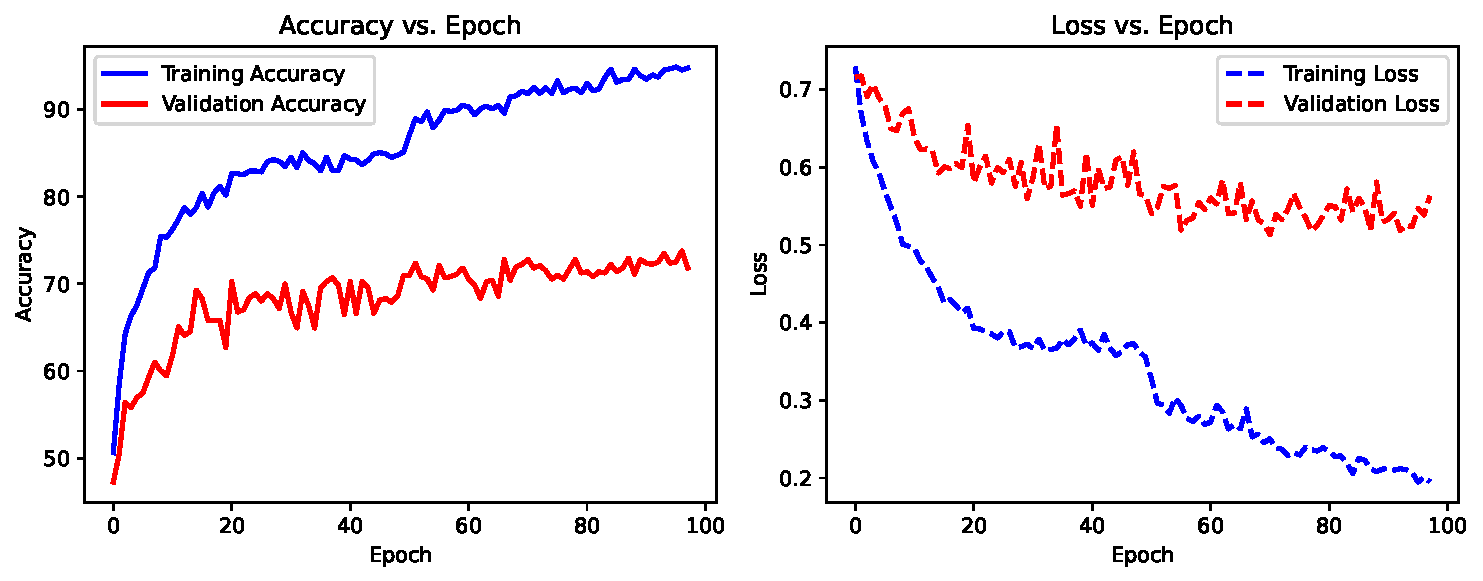
\includegraphics[width=0.45\textwidth]{vis_pdf/TCC_model_perf.pdf}
    \caption{TCC Training (Speaker Dependent - DAIC)}
    \label{fig:training_TCC_daic}
\end{figure}



